% questions.tex —— 2004 年·普通高等学校招生考试·湖南卷·理科 · 题目内容片段（无答案）
% 由 tools/generate_projects.py 依来源总账自 2004/2004_数学真题_湖南理科_试题.md 生成，勿手改（改源 MD 后重跑）

\gkpart{一、选择题：本大题共 12 小题，每小题 5 分，共 60 分．在每小题给出的四个选项中，只有一项是符合题目要求的．}

\begin{question}
\gkti{1}复数 $\left(1 + \dfrac{1}{\mathrm{i}}\right)^4$ 的值是\mbox{（　　）}

\begin{gkopts}(4)
\task A．$4\mathrm{i}$
\task B．$-4\mathrm{i}$
\task C．$4$
\task D．$-4$
\end{gkopts}

\end{question}
\begin{question}
\gkti{2}如果双曲线 $\dfrac{x^2}{13} - \dfrac{y^2}{12} = 1$ 上一点 $P$ 到右焦点的距离等于 $\sqrt{13}$，那么点 $P$ 到右准线的距离是\mbox{（　　）}

\begin{gkopts}(4)
\task A．$\dfrac{13}{5}$
\task B．$13$
\task C．$5$
\task D．$\dfrac{5}{13}$
\end{gkopts}

\end{question}
\begin{question}
\gkti{3}设 $f^{-1}(x)$ 是函数 $f(x) = \log_2(x + 1)$ 的反函数，若 $[1 + f^{-1}(a)][1 + f^{-1}(b)] = 8$，则 $f(a + b)$ 的值为\mbox{（　　）}

\begin{gkopts}(4)
\task A．$1$
\task B．$2$
\task C．$3$
\task D．$\log_2 3$
\end{gkopts}

\end{question}
\begin{question}
\gkti{4}把正方形 $ABCD$ 沿对角线 $AC$ 折起，当以 $A, B, C, D$ 四点为顶点的三棱锥体积最大时，直线 $BD$ 和平面 $ABC$ 所成的角的大小为\mbox{（　　）}

\begin{gkopts}(4)
\task A．$90^\circ$
\task B．$60^\circ$
\task C．$45^\circ$
\task D．$30^\circ$
\end{gkopts}

\end{question}
\begin{question}
\gkti{5}某公司在甲、乙、丙、丁四个地区分别有 $150$ 个、$120$ 个、$180$ 个、$150$ 个销售点．公司为了调查产品销售的情况，需从这 $600$ 个销售点中抽取一个容量为 $100$ 的样本，记这项调查为①；在丙地区中有 $20$ 个特大型销售点，要从中抽取 $7$ 个调查其销售收入和售后服务情况，记这项调查为②．则完成①、②这两项调查宜采用的抽样方法依次是\mbox{（　　）}

\begin{gkopts}(2)
\task A．分层抽样，系统抽样法
\task B．分层抽样法，简单随机抽样法
\task C．系统抽样法，分层抽样法
\task D．简随机抽样法，分层抽样法
\end{gkopts}

\end{question}
\begin{question}
\gkti{6}设函数 $f(x) = \begin{cases} x^2 + bx + c, & x \leqslant 0, \\ 2, & x > 0. \end{cases}$ 若 $f(-4) = f(0)$，$f(-2) = -2$，则关于 $x$ 的方程 $f(x) = x$ 的解的个数为\mbox{（　　）}

\begin{gkopts}(4)
\task A．$1$
\task B．$2$
\task C．$3$
\task D．$4$
\end{gkopts}

\end{question}
\begin{question}
\gkti{7}设 $a > 0$，$b > 0$，则以下不等式中不恒成立的是\mbox{（　　）}

\begin{gkopts}(1)
\task A．$(a + b)\left(\dfrac{1}{a} + \dfrac{1}{b}\right) \geqslant 4$
\task B．$a^3 + b^3 \geqslant 2ab^2$
\task C．$a^2 + b^2 + 2 \geqslant 2a + 2b$
\task D．$\sqrt{|a - b|} \geqslant \sqrt{a} - \sqrt{b}$
\end{gkopts}

\end{question}
\begin{question}
\gkti{8}数列 $\{a_n\}$ 中，$a_1 = \dfrac{1}{5}$，$a_n + a_{n+1} = \dfrac{6}{5^{n+1}}$，$n \in \mathbf{N}^*$，则 $\lim\limits_{n \to \infty} (a_1 + a_2 + \cdots + a_n) =$\mbox{（　　）}

\begin{gkopts}(4)
\task A．$\dfrac{2}{5}$
\task B．$\dfrac{2}{7}$
\task C．$\dfrac{1}{4}$
\task D．$\dfrac{4}{25}$
\end{gkopts}

\end{question}
\begin{question}
\gkti{9}设集合 $U = \{(x, y) \mid x \in \mathbf{R}, y \in \mathbf{R}\}$，$A = \{(x, y) \mid 2x - y + m > 0\}$，$B = \{(x, y) \mid x + y - n \leqslant 0\}$，那么点 $P(2, 3) \in A \cap (\complement_U B)$ 的充要条件是\mbox{（　　）}

\begin{gkopts}(4)
\task A．$m > -1, n < 5$
\task B．$m < -1, n < 5$
\task C．$m > -1, n > 5$
\task D．$m < -1, n > 5$
\end{gkopts}

\end{question}
\begin{question}
\gkti{10}从正方体的八个顶点中任取三个点为顶点作三角形，其中直角三角形的个数为\mbox{（　　）}

\begin{gkopts}(4)
\task A．$56$
\task B．$52$
\task C．$48$
\task D．$40$
\end{gkopts}

\end{question}
\begin{question}
\gkti{11}农民收入由工资性收入和其它收入两部分构成．2003 年某地区农民人均收入为 $3150$ 元（其中工资性收入为 $1800$ 元，其它收入为 $1350$ 元），预计该地区自 2004 年起的 $5$ 年内，农民的工资性收入将以每年 $6\%$ 的年增长率增长，其它收入每年增加 $160$ 元．根据以上数据，2008 年该地区农民人均收入介于\mbox{（　　）}

\begin{gkopts}(2)
\task A．$4200$ 元 $\sim 4400$ 元
\task B．$4400$ 元 $\sim 4600$ 元
\task C．$4600$ 元 $\sim 4800$ 元
\task D．$4800$ 元 $\sim 5000$ 元
\end{gkopts}

\end{question}
\begin{question}
\gkti{12}设 $f(x)$、$g(x)$ 分别是定义在 $\mathbf{R}$ 上的奇函数和偶函数，当 $x < 0$ 时，$f'(x)g(x) + f(x)g'(x) > 0$，且 $g(-3) = 0$，则不等式 $f(x)g(x) < 0$ 的解集是\mbox{（　　）}

\begin{gkopts}(2)
\task A．$(-3, 0) \cup (3, +\infty)$
\task B．$(-3, 0) \cup (0, 3)$
\task C．$(-\infty, -3) \cup (3, +\infty)$
\task D．$(-\infty, -3) \cup (0, 3)$
\end{gkopts}

\end{question}
\gkpart{二、填空题：本大题共 4 小题，每小题 4 分，共 16 分．把答案填在横线上．}

\begin{question}
\gkti{13}已知向量 $\vec{a} = (\cos\theta, \sin\theta)$，向量 $\vec{b} = (\sqrt{3}, -1)$，则 $|2\vec{a} - \vec{b}|$ 的最大值是 $\underline{\hspace{2cm}}$．

\end{question}
\begin{question}
\gkti{14}同时抛掷两枚相同的均匀硬币，随机变量 $\xi = 1$ 表示结果中有正面向上，$\xi = 0$ 表示结果中没有正面向上，则 $E\xi = \underline{\hspace{2cm}}$．

\end{question}
\begin{question}
\gkti{15}若 $\left(x^3 + \dfrac{1}{x\sqrt{x}}\right)^n$ 的展开式中的常数项为 $84$，则 $n = \underline{\hspace{2cm}}$．

\end{question}
\begin{question}
\gkti{16}设 $F$ 是椭圆 $\dfrac{x^2}{7} + \dfrac{y^2}{6} = 1$ 的右焦点，且椭圆上至少有 $21$ 个不同的点 $P_i$ ($i = 1, 2, 3, \cdots$)，使 $|FP_1|, |FP_2|, |FP_3|, \cdots$ 组成公差为 $d$ 的等差数列，则 $d$ 的取值范围为 $\underline{\hspace{2cm}}$．

\end{question}
\gkpart{三、解答题：本大题共 6 小题，共 74 分．解答应写出文字说明、证明过程或演算步骤．}

\begin{question}
\gkti{17}（本小题满分 12 分）

已知 $\sin\left(\dfrac{\pi}{4} + 2\alpha\right) \cdot \sin\left(\dfrac{\pi}{4} - 2\alpha\right) = \dfrac{1}{4}$，$\alpha \in \left(\dfrac{\pi}{4}, \dfrac{\pi}{2}\right)$，求 $2\sin^2\alpha + \tan\alpha - \cot\alpha - 1$ 的值．

\Needspace{0.4\textheight}
\end{question}
\begin{question}
\gkti{18}（本小题满分 12 分）

如图，在底面是菱形的四棱锥 $P - ABCD$ 中，$\angle ABC = 60^\circ$，$PA = AC = a$，$PB = PD = \sqrt{2}a$，点 $E$ 在 $PD$ 上，且 $PE : ED = 2 : 1$．
\nopagebreak[4]
\begin{center}% Source-faithful schematic draft: 2004 Hunan Science Q18, PDF p.1 (printed p.174).
% Source ID: src-9f80071b553ab4b942482c92509eda24ffc4990bd51cd38172372a29634438da
% Source SHA-256: 47ba4497f88a0667fcfd694f4b8a9a37e7b1d3f098a0ad26b0529b990194e2c7
\begin{tikzpicture}[line width=0.6pt,scale=1.1,every node/.style={inner sep=1.5pt}]
  % Coordinates of pyramid P-ABCD with rhombus base ABCD
  % A is behind, PA is perpendicular to base ABCD
  \coordinate (A) at (0, 0);
  \coordinate (B) at (-1.8, -0.9);
  \coordinate (C) at (0.2, -1.5);
  \coordinate (D) at (2.0, 0);
  \coordinate (P) at (0, 2.5);
  \coordinate (E) at ($(P)!0.6667!(D)$);

  % Dashed interior lines
  \draw[dashed, line width=0.5pt] (P) -- (A);
  \draw[dashed, line width=0.5pt] (A) -- (B);
  \draw[dashed, line width=0.5pt] (A) -- (D);
  \draw[dashed, line width=0.5pt] (A) -- (C);
  \draw[dashed, line width=0.5pt] (A) -- (E);

  % Solid exterior edges and section lines
  \draw (P) -- (B);
  \draw (P) -- (D);
  \draw (B) -- (C);
  \draw (C) -- (D);
  \draw (E) -- (C);

  % Vertex labels faithful to original layout
  \node[above] at (P) {$P$};
  \node[above left] at (A) {$A$};
  \node[below left] at (B) {$B$};
  \node[below] at (C) {$C$};
  \node[right] at (D) {$D$};
  \node[above right] at (E) {$E$};
\end{tikzpicture}
\end{center}
\nopagebreak[4]
(1) 证明：$PA \perp$ 平面 $ABCD$；

(2) 求以 $AC$ 为棱，$EAC$ 与 $DAC$ 为面的二面角 $\theta$ 的大小；

(3) 在棱 $PC$ 上是否存在一点 $F$，使 $BF \parallel$ 平面 $AEC$？证明你的结论．

\end{question}
\begin{question}
\gkti{19}（本小题满分 12 分）

甲、乙、丙三台机床各自独立地加工同一种零件，已知甲机床加工的零件是一等品而乙机床加工的零件不是一等品的概率为 $\dfrac{1}{4}$，乙机床加工的零件是一等品而丙机床加工的零件不是一等品的概率为 $\dfrac{1}{12}$，甲、丙两台机床加工的零件都是一等品的概率为 $\dfrac{2}{9}$．

(1) 分别求甲、乙、丙三台机床各自加工零件是一等品的概率；

(2) 从甲、乙、丙加工的零件中各取一个检验，求至少有一个一等品的概率．

\end{question}
\begin{question}
\gkti{20}（本小题满分 12 分）

已知函数 $f(x) = x^2 \mathrm{e}^{ax}$，其中 $a \leqslant 0$，$\mathrm{e}$ 为自然对数的底数．

(1) 讨论函数 $f(x)$ 的单调性；

(2) 求函数 $f(x)$ 在区间 $[0, 1]$ 上的最大值．

\Needspace{0.4\textheight}
\end{question}
\begin{question}
\gkti{21}（本小题满分 13 分）

如图，过抛物线 $x^2 = 4y$ 的对称轴上任一点 $P(0, m)$ ($m > 0$) 作直线与抛物线交于 $A, B$ 两点，点 $Q$ 是点 $P$ 关于原点的对称点．
\nopagebreak[4]
\begin{center}% Source-faithful schematic draft: 2004 Hunan Science Q21, PDF p.2 (printed p.175).
% Source ID: src-9f80071b553ab4b942482c92509eda24ffc4990bd51cd38172372a29634438da
% Source SHA-256: 47ba4497f88a0667fcfd694f4b8a9a37e7b1d3f098a0ad26b0529b990194e2c7
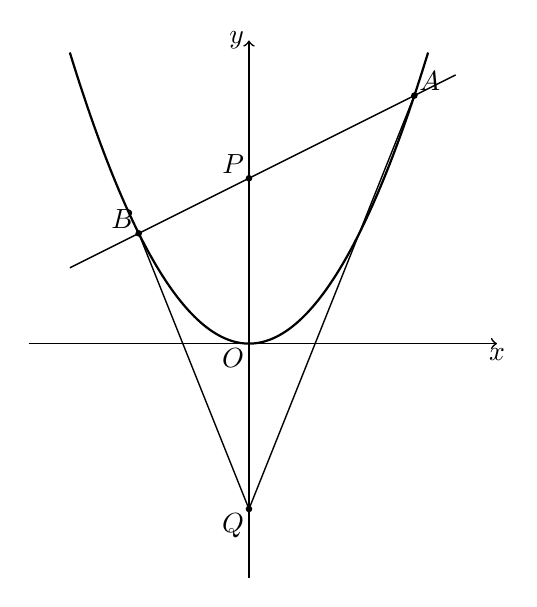
\begin{tikzpicture}[line width=0.6pt,scale=0.35,every node/.style={inner sep=1.5pt}]
  % Axes
  \draw[->] (-8, 0) -- (9, 0) node[below] {$x$};
  \draw[->] (0, -8.5) -- (0, 11) node[left] {$y$};
  \node[below left] at (0, 0) {$O$};

  % Parabola x^2 = 4y => y = x^2 / 4
  \draw[thick,domain=-6.5:6.5,samples=60,smooth] plot (\x, {0.25*\x*\x});

  % Points P(0, 6) and Q(0, -6)
  \coordinate (P) at (0, 6);
  \coordinate (Q) at (0, -6);
  \fill (P) circle (0.12) node[above left] {$P$};
  \fill (Q) circle (0.12) node[below left] {$Q$};

  % Points A(6, 9) and B(-4, 4) on parabola and line y = 0.5x + 6
  \coordinate (A) at (6, 9);
  \coordinate (B) at (-4, 4);
  \fill (A) circle (0.12) node[above right] {$A$};
  \fill (B) circle (0.12) node[above left] {$B$};

  % Secant line AB passing through P
  \draw[line width=0.55pt] (-6.5, 2.75) -- (7.5, 9.75);

  % Lines QA and QB
  \draw[line width=0.5pt] (Q) -- (A);
  \draw[line width=0.5pt] (Q) -- (B);
\end{tikzpicture}
\end{center}
\nopagebreak[4]
(1) 设点 $P$ 分有向线段 $\vec{AB}$ 所成的比为 $\lambda$，证明：$\vec{QP} \perp (\vec{QA} - \lambda\vec{QB})$；

(2) 设直线 $AB$ 的方程是 $x - 2y + 12 = 0$，过 $A, B$ 两点的圆 $C$ 与抛物线在点 $A$ 处有共同的切线，求圆 $C$ 的方程．

\Needspace{0.4\textheight}
\end{question}
\begin{question}
\gkti{22}（本小题满分 13 分）

如图，直线 $l_1: y = kx + 1 - k$ $\left(k \neq 0, k \neq \pm \dfrac{1}{2}\right)$ 与 $l_2: y = \dfrac{1}{2}x + \dfrac{1}{2}$ 相交于点 $P$．直线 $l_1$ 与 $x$ 轴交于点 $P_1$，过点 $P_1$ 作 $x$ 轴的垂线交直线 $l_2$ 于点 $Q_1$，过点 $Q_1$ 作 $y$ 轴的垂线交直线 $l_1$ 于点 $P_2$，过点 $P_2$ 作 $x$ 轴的垂线交直线 $l_2$ 于点 $Q_2$，$\cdots$，这样一直作下去，可得到一系列点 $P_1, Q_1, P_2, Q_2, \cdots$．点 $P_n$ ($n = 1, 2, \cdots$) 的横坐标构成数列 $\{x_n\}$．
\nopagebreak[4]
\begin{center}% Source-faithful schematic draft: 2004 Hunan Science Q22, PDF p.2 (printed p.175).
% Source ID: src-9f80071b553ab4b942482c92509eda24ffc4990bd51cd38172372a29634438da
% Source SHA-256: 47ba4497f88a0667fcfd694f4b8a9a37e7b1d3f098a0ad26b0529b990194e2c7
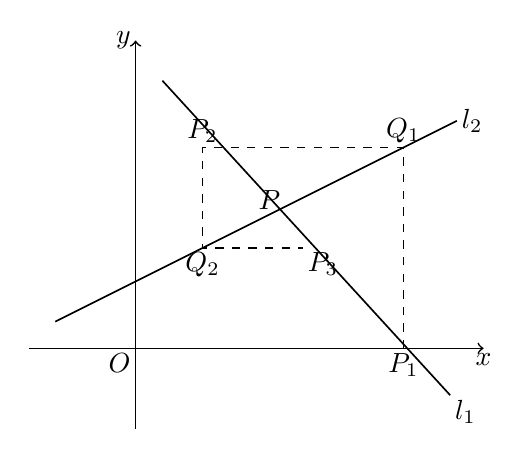
\begin{tikzpicture}[line width=0.6pt,scale=1.7,every node/.style={inner sep=1.5pt}]
  % Axes
  \draw[->] (-0.8, 0) -- (2.6, 0) node[below] {$x$};
  \draw[->] (0, -0.6) -- (0, 2.3) node[left] {$y$};
  \node[below left] at (0, 0) {$O$};

  % Coordinates based on k = -1:
  % P(1, 1), l1: y = -x + 2, l2: y = 0.5x + 0.5
  \coordinate (P) at (1, 1);
  \coordinate (P1) at (2, 0);
  \coordinate (Q1) at (2, 1.5);
  \coordinate (P2) at (0.5, 1.5);
  \coordinate (Q2) at (0.5, 0.75);
  \coordinate (P3) at (1.25, 0.75);

  % Line l1
  \draw[line width=0.6pt] (0.2, 2.0) -- (2.35, -0.35) node[below right] {$l_1$};

  % Line l2
  \draw[line width=0.6pt] (-0.6, 0.2) -- (2.4, 1.7) node[right] {$l_2$};

  % Dashed staircase lines
  \draw[dashed, line width=0.5pt] (P1) -- (Q1) -- (P2) -- (Q2) -- (P3);

  % Labels
  \node[above] at (P) {$P$};
  \node[below] at (P1) {$P_1$};
  \node[above] at (Q1) {$Q_1$};
  \node[above] at (P2) {$P_2$};
  \node[below] at (Q2) {$Q_2$};
  \node[below right] at (P3) {$P_3$};
\end{tikzpicture}
\end{center}
\nopagebreak[4]
(1) 证明：$x_{n+1} - 1 = \dfrac{1}{2k}(x_n - 1)$，$n \in \mathbf{N}^*$；

(2) 求数列 $\{x_n\}$ 的通项公式；

(3) 比较 $2|PP_n|^2$ 与 $4k^2|PP_1|^2 + 5$ 的大小．

\end{question}